\chapter{Implementación hardware del robot}
\label{cap:capitulo5}

\begin{flushright}
\begin{minipage}[]{10cm}
\emph{La perfección se logra no cuando no hay nada más que añadir, sino cuando no hay nada más que quitar}\\
\end{minipage}\\

Antoine de Saint-Exupéry\\
\end{flushright}

\vspace{1cm}

Tras haber expuesto todas las plataformas de desarrollo utilizadas en este proyecto, en este capítulo se describirá el proceso paso a paso, desde la concepción inicial hasta la construcción y ensamblaje, para que sea completamente operativo el robot.

\section{Geometría del robot}

En este apartado se detalla el proceso llevado a cabo para definir la idea y la forma elegida para el robot.

La aplicación de este proyecto se encuentra dentro de los robots de campo y es por ello que estos tipos de robots son plataformas que trabajan en entornos no estructurados, como se comentó en el Capítulo 1. Por ello, es necesario que la estructura del robot se asemeje a esos tipos de robots y los más comunes son los robots con ruedas. 

Sin embargo los robots de campo son de gran coste y grandes dimensiones, lo que hacía inviable que entidades con recursos limitados pudieran adquirirlos. Es por ello que se decidió apostar por los robots de bajo coste y gracias a mi tutor Julio Vega y a su Pibot pude centrarme en encontrar la solución final a mi proyecto. 

Pibot es un proyecto descrito en \ref , trata de un robot de bajo coste (resumir lo del paper). Otra aplicación que ha encontrado es (nombrar el otro paper y una breve descripción)

(incluir foto del robot) 


Tiene los siguientes grados de libertad ... (incluir foto con ellos), dim 20x10x8 cm
Para poder empezar a trabajar se decidió usar una pieza de aluminio para cambiar la disposición de la cámara y mirase para abajo.

LA IDEA DE TENER QUE EL ROBOT FUERA ASÍ: 

Describir la disposición geométrica de los sensores y cámaras, cubriendo su campo de visión, ángulo de captura o alcance. (espacio del trabajo aplicado al robot), simetría del roboT


Los grados de libertad, centro de gravedad y explicar cómo es la estabilidad.

ADAPTÉ AL PIBOT  PARA QUE CUMPLIESE CON EL OBJETIVO PRINCIPAL DEL CAPÍTULO 3 


A LO MEJOR HACER UN APARTADO PARA EL ESQUELETO DEL ROBOT 

Finalmente para poder cumplir con el objetivo principal es necesario definir el esqueleto del robot, los componentes electromecánicos, todos aquellos que no se pueden imprimir. 

Distribuir los componentes (foto de fritzing): motores, sensores, cámaras (fotos mías)



\section{Elección de componentes hardware}

Explicar todos los componentes usados: 

Si se incluyen imágenes que sean distintas a las del apartado de plataformas de desarrollo o no incluirlas. 

Fotos hechas por mí 

Uso las características que he aprovechado del capítulo 4 

\subsection{Raspberry Pi}

Es muy usado en robótica, ordenador a bordo,....

\subsection{Servomotores Parallax}
La fuerza, la utilidad que hacen,...


\subsection{Ruedas ActivityBot}
La fuerza, la utilidad que hacen,...

\subsection{Rueda/Bola Loca}
La fuerza, la utilidad que hacen,...

\subsection{Raspberry Pi Cámara}

Calidad de la imagen, parámetros intrínsecos teóricos,... 

\subsection{GPS NEO 6M}
Explicar el módulo GPS .... pruebas, alcance... tarda en coger señal, la luz azul...

\subsection{Google Coral USB}

Utilidades, el nivel de cómputo que llega,... inferencias por segundo,tipo de modelos compatible...

\subsection{Powerbank}
 
 Todo el día encendida y ejecutando, aguanta perfectamente... 
 
  
\section{Bocetos}

incluir los bocetos hechos a papel

incluir la maqueta creada con cartón ya que no disponía de una impresora 3D

\section{Diseño CAD}

Incluir imágenes de los planos, de las piezas con las medidas,...

Se decidió dividir en 4 piezas que tienen distintas finalidades:

\subsection{Pieza base}
Esta parte es la que se encuentran los motores de las ruedas y de la cámara. También, he diseñado un rectángulo para poner la rueda loca que va pegada.

Los 4 rectángulos que hay en los lados de la parte superior, se usa para poder pasar los cables y que no quede feo estéticamente desde fuera. Los 4 círculos son para poner posteriormente los tornillos y sujetar la parte superior.

\subsection{Pieza cámara}
La cámara va sujeta de forma diagonal, ya que no hace falta poner los 4 tornillos. Esto ocure tanto en la parte de la cámara como en la base del servo que usa.


\subsection{Pieza sujección trasera}
He creado esta prolongación que va fija con un tornillo para evitar que la batería se salga si el terreno no es regular. Tras imprimir y ensamblar la pieza, ha quedado así:

\subsection{Pieza batería}

Esta pieza está diseñada para alojar en su interior una powerbank y he cread unas aberturas para poder sacar la powerbank cuando sea necesaria.

Los huecos laterale son para almacenar los cables y poder unir esta pieza con la base.

En su parte superior, hay 12 agujeros para poder ensamblar con tornillos: raspberry pi, módulo GPS y la antena.



\section{Impresión y montaje}


Dificultades imprimiendo: con la impresora del instituto. Incluir características de la impresora y de la impresión usada.

Impresión de Gonzalo
Características: 

Impresora FDM Creality Ender3 V2
Slicer Software: UltiMaker Cura

QUALITY:
Layer height: 0.2 mm
Line width: 0.4 mm

WALLS: 
Wall thickness: 0.8 mm
Wall line count: 2
Z sean alignment: "Sharpest corner"
Seam corner preference: "Smart hiding"

INFILL:
Infill density: 15%
Infill pattern: "Gyroid"

SPEED:
Print speed: 50 mm/s
Initial layer speed: 20 mm/s


Incluir una lista de los tornillos usados, hama  beads...\\\\



Incluir imagen completa que incluya el Google Coral USB\\\\\\


INCLUIR MUCHAS FOTOS\\\\\\


\section{Snippets}

Puede resultar interesante, para clarificar la descripción, mostrar fragmentos de código (o \textit{snippets}) ilustrativos. En el Código \ref{cod:codejemplo} vemos un ejemplo escrito en \texttt{C++}.

\begin{code}[h]
\begin{lstlisting}[language=C++]
void Memory::hypothesizeParallelograms () {
  for(it1 = this->controller->segmentMemory.begin(); it1++) {
    squareFound = false; it2 = it1; it2++;
    while ((it2 != this->controller->segmentMemory.end()) && (!squareFound)) {
      if (geometry::haveACommonVertex((*it1),(*it2),&square)) {
        dist1 = geometry::distanceBetweenPoints3D ((*it1).start, (*it1).end);
        dist2 = geometry::distanceBetweenPoints3D ((*it2).start, (*it2).end);
      }
    // [...]
\end{lstlisting}
\caption[Función para buscar elementos 3D en la imagen]{Función para buscar elementos 3D en la imagen}
\label{cod:codejemplo}
\end{code}

En el Código \ref{cod:codejemplo2} vemos un ejemplo escrito en \texttt{Python}.

\begin{code}[h]
\begin{lstlisting}[language=Python]
def mostrarValores():
    print (w1.get(), w2.get())

master = Tk()
w1 = Scale(master, from_=0, to=42)
w1.pack()
w2 = Scale(master, from_=0, to=200, orient=HORIZONTAL)
w2.pack()
Button(master, text='Show', command=mostrarValores).pack()

mainloop()
\end{lstlisting}
\caption[Cómo usar un Slider]{Cómo usar un Slider}
\label{cod:codejemplo2}
\end{code}

\section{Verbatim}

Para mencionar identificadores usados en el código ---como nombres de funciones o variables--- en el texto, usa el entorno literal o verbatim \verb|hypothesizeParallelograms()|. También se puede usar este entorno para varias líneas, como se ve a continuación:

\begin{verbatim}
void Memory::hypothesizeParallelograms () {
  // add your code here
}
\end{verbatim}

\section{Ecuaciones}

Si necesitas insertar alguna ecuación, puedes hacerlo. Al igual que las figuras, no te olvides de referenciarlas. A continuación se exponen algunas ecuaciones de ejemplo: Ecuación \ref{ec:ec1} y Ecuación \ref{ec:ec2}.

\begin{myequation}[h]
\begin{equation}
H = 1 - \frac{\sum_{i=0}^{N}\frac{(\frac{d_{j_s} + d_{j_e}}{2})}{N}}{M}
\nonumber
\label{ec:ec1}
\end{equation}
\caption[Ejemplo de ecuación con fracciones]{Ejemplo de ecuación con fracciones}
\end{myequation} 

\begin{myequation}[h]
\begin{equation}
v(entrada)= \left\{
	\begin{array}{lcc}
		0 & \mbox{if} & \epsilon_t < 0.1\\
		K_p\cdot{(T_{t}-T)} & \mbox{if}& 0.1 \leq \epsilon_t < M_t\\
		K_p \cdot M_t & \mbox{if}& M_t < \epsilon_t
	\end{array}
\right.
\label{ec:ec2}
\end{equation}
\caption[Ejemplo de ecuación con array y letras y símbolos especiales]{Ejemplo de ecuación con array y letras y símbolos especiales}
\end{myequation}

\section{Tablas o cuadros}

Si necesitas insertar una tabla, hazlo dígnamente usando las propias tablas de \LaTeX, no usando pantallazos e insertándolas como figuras... En el Cuadro \ref{cuadro:ejemplo} vemos un ejemplo.

\begin{table}[H]
\begin{center}
\begin{tabular}{|c|c|}
\hline
\textbf{Parámetros} & \textbf{Valores} \\
\hline
Tipo de sensor & Sony IMX219PQ[7] CMOS 8-Mpx \\
Tamaño del sensor & 3.674 x 2.760 mm (1/4" format) \\
Número de pixels & 3280 x 2464 (active pixels) \\
Tamaño de pixel & 1.12 x 1.12 um \\
Lente & f=3.04 mm, f/2.0 \\
Ángulo de visión & 62.2 x 48.8 degrees \\
Lente SLR equivalente & 29 mm \\
\hline
\end{tabular}
\caption{Parámetros intrínsecos de la cámara}
\label{cuadro:ejemplo}
\end{center}
\end{table}

En los textos puedes poner palabras en \textit{cursiva}, para aquellas expresiones en sentido \textit{figurado}, palabras como \textit{robota}, que está fuera del diccionario castellano, o bien para resaltar palabras de una colección: \textit{(a)} es la primera letra del abecedario, \textit{(b)} es la segunda, etc.\\

Al poner las dos líneas del anterior párrafo, este aparecerá separado del anterior. Si no las pongo, los párrafos aparecerán pegados. Sigue el criterio que consideres más oportuno.

\section{Segunda sección}
\label{sec:segundaseccion}

No olvides incluir imágenes y referenciarlas, como la Figura \ref{fig:roomba}.

\begin{figure} [h!]
	\begin{center}
		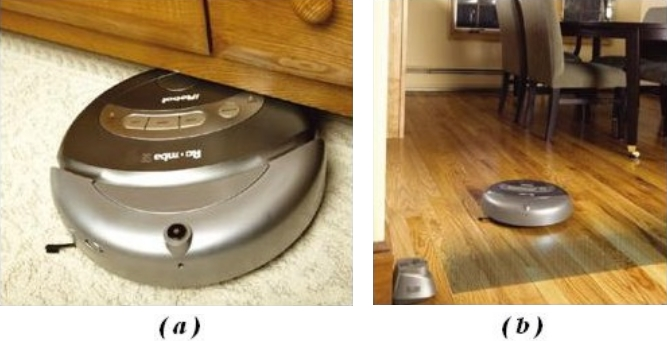
\includegraphics[width=8cm]{figs/roomba}
	\end{center}
	\caption{Robot aspirador Roomba de iRobot.}
	\label{fig:roomba}
\end{figure}\

Ni tampoco olvides de poner las URLs como notas al pie. Por ejemplo, si hablo de la Robocup\footnote{\url{http://www.robocup.org}}.

\subsection{Números}
\label{sec:subseccion}

En lugar de tener secciones interminables, como la Sección \ref{sec:robotica}, divídelas en subsecciones.

Para hablar de números, mételos en el entorno \textit{math} de \LaTeX, por ejemplo, $1.5Kg$. También puedes usar el símbolo del Euro como aquí: 1.500\euro.

\subsection{Listas}

Cuando describas una colección, usa \texttt{itemize} para ítems o \texttt{enumerate} para enumerados. Por ejemplo:

\begin{itemize}
	\item \textit{Entorno de simulación.} Hemos usado dos entornos de simulación: uno en 3D y otro en 2D.
	\item \textit{Entornos reales.} Dentro del campus, hemos realizado experimentos en Biblioteca y en el edificio de Gestión.
\end{itemize}\

\begin{enumerate}
	\item Primer elemento de la colección.
	\item Segundo elemento de la colección.
\end{enumerate}\

\paragraph{Referencias bibliográficas}
\label{sec:referencias}

Cita, sobre todo en este capítulo, referencias bibliográficas que respalden tu argumento. Para citarlas basta con poner la instrucción \verb|\cite| con el identificador de la cita. Por ejemplo: libros como \cite{vega12e}, artículos como \cite{vega19b}, URLs como \cite{vega19a}, tesis como \cite{vega18b}, congresos como \cite{vega18a}, u otros trabajos fin de grado como \cite{vega08b}.

Las referencias, con todo su contenido, están recogidas en el fichero \texttt{bibliografia.bib}. El contenido de estas referencias está en formato \texttt{BibTex}. Este formato se puede obtener en muchas ocasiones directamente, desde plataformas como \texttt{Google Scholar} u otros repositorios de recursos científicos.

Existen numerosos estilos para reflejar una referencia bibliográfica. El estilo establecido por defecto en este documento es APA, que es uno de los estilos más comunes, pero lo puedes modificar en el archivo \texttt{memoria.tex}; concretamente, cambiando el campo \verb|apalike| a otro en la instrucción \verb|\bibliographystyle{apalike}|. 

\

\

\

Y, para terminar este capítulo, resume brevemente qué vas a contar en los siguientes.
